\section*{\centering Kastparabel med och utan luftmotstånd}

Utan luftmotstånd...
\begin{equation} \label{eq:xyt}
    \begin{cases}
        x(t) = x_0 + v_{0,x}t \\
        y(t) = y_0 + v_{0,y}t - \dfrac{1}{2}gt^2
    \end{cases}
\end{equation}
Anta att startpunkt ($x_0$,$y_0$) ligger i (0,0) och separera $v_0$ 
\begin{align}
    x(t) &= v_0cos\theta t \label{eq:xt}\\
    y(t) &= v_0sin\theta t - \dfrac{1}{2}gt^2 \label{eq:yt}
\end{align}

\begin{figure}[H]
    \centering
    \captionsetup{justification=centering,margin=2cm}
    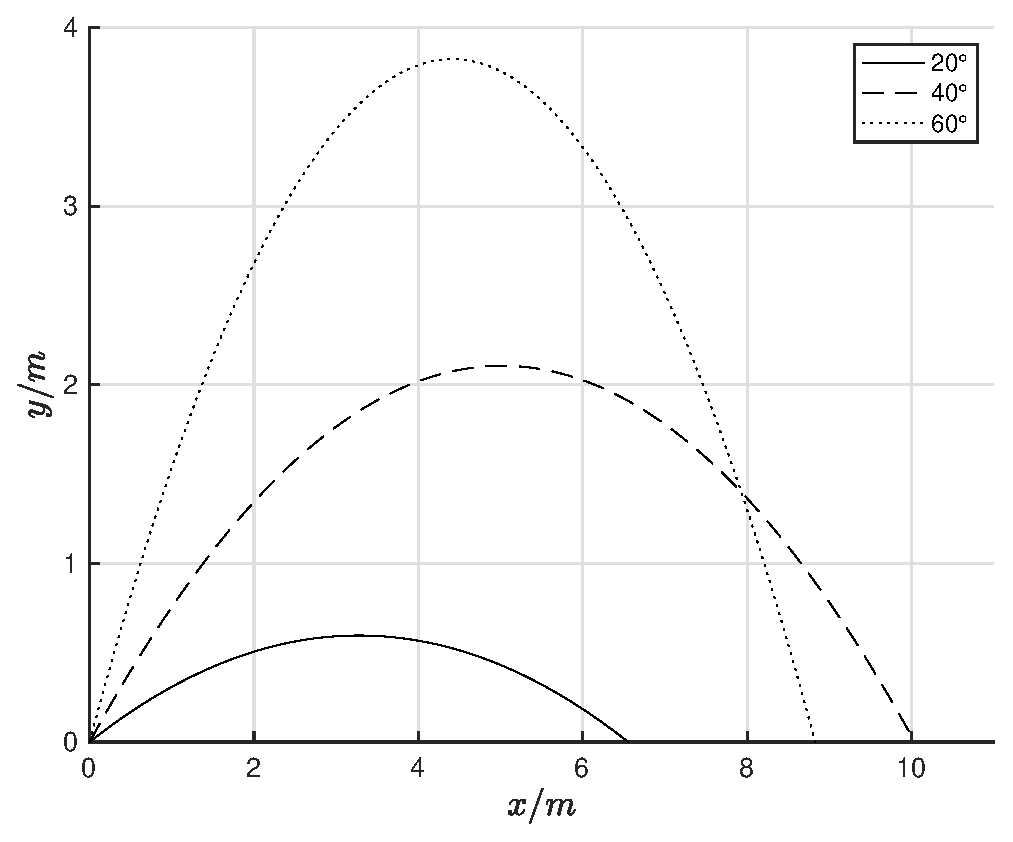
\includegraphics[scale=0.5]{Resources/Graphics/fig2_1.eps}
    \caption{Utan luftmotstånd}
    \label{fig:2_1}
\end{figure}

% Problem 2b
\np 
Med luftmotstånd: 
\begin{align}
    a_x = \dfrac{dv_x}{dt} &= -kv_x \label{eq:2b_ax}\\
    a_y = \dfrac{dv_y}{dt} &= -kv_y -g \label{eq:2b_ay}
\end{align}
Efter integration av $a_x$ och $a_y$:


\begin{align} 
    v_x(t) = \dfrac{dx}{dt} &= v_{0,x}e^{-kt} \label{eq:2b_vx} \\ 
    v_y(t) = \dfrac{dy}{dt} &= v_{0,y}e^{-kt}- \dfrac{g}{k}
    \label{eq:2b_vy}
\end{align}

var $v_{0,x}$ är $v_0 \text{cos}\theta$  och  $v_{0,y}$ är $v_0 \text{sin}\theta$ sätts in och integreras

\begin{align} 
    x(t) &= \dfrac{v_0 \text{cos}\theta}{k}\left( 1-e^{-kt} \right) \\
    y(t) &= \dfrac{1}{k}\left( \left(v_0\text{sin}\theta + \frac{g}{k}\right)(1-e^{-kt}) -gt \right) \label{eq:2b_y}
\end{align}

\np
\subsection*{MatLab kod}
\lstinputlisting[caption={\quad}] {Resources/Code/2.m}